	\documentclass[a4paper,12pt]{report}

\usepackage{graphicx}
\usepackage{pgfplots}
\usepackage{graphicx}
\usepackage{hyperref}
\usepackage{alltt, fancyvrb, url}
\usepackage[utf8]{inputenc}
\usepackage{float}

\pgfplotsset{compat=1.18}

\title{
\includegraphics[width=\textwidth]{res/logoInverted.pdf}
\\ \textbf {Report}}

\author{Pietro Olivi\\
Leonardo Tassinari\\
Lorenzo Dalmonte}
\date{\today}


\begin{document}

\maketitle

\tableofcontents

\chapter{Analysis}
The software aims to create an application designed to enhance psycho-motor skills through a gaming experience based on multitasking.\\
The term \textit{Multitasking} refers to the ability of a person or a product to do more than one thing at a time.

\section{Requirements}
\subsection*{Functional}
\begin{itemize}
	\item Upon starting, the software will display a simple minigame.\footnote{A minigame is a potentially-never-ending challenge that requires simple actions from the player in order to keep the game going.}
	\item After a short amount of time a new minigame will appear and so on until all four minigames are shown.
	\item Generally, the difficulty of each minigame shall increase over time.
	\item The player's goal is to survive as long as possible. After failing any minigame the application will display the final result,
	      therefore the software has to keep track of how long the player has lasted in the current run in order to calculate the score.
	\item It will be possible to appreciate the improvement on a \textit{Statistics} page that will show the record of all the past runs.
\end{itemize}

\subsection*{Non-functional}
\begin{itemize}
	\item The application shall sustain acceptable frame rate (around 60 fps) in all the sections of the gameplay, even on older hardware\footnote{e.g. Intel Core i5 (fourth generation), 8Gb of RAM.}.
	\item For Developers shall be possible to easily develop and swap the\\ minigames among the ones that best fit the training purposes of the user on top of those already provided.
	\item It shall be possible to play in full screen mode.
	\item The window shall be resizable to fit in any kind of screen\footnote{Provided a minimum resolution.}.
\end{itemize}



\section{Domain analysis}

MTSK-Game must exhibit some \textit{minigames}, the ones supplied by us are:
\begin{itemize}
	\item \textit{WhacAMole}: where the goal is to crush all the moles that emerge from the dens, before they re-enter them, avoiding to detonate bombs that will also pop up from the burrows.
	\item \textit{DodgeATriangle}: in which the player has to slide a \textit{rectangle} up and down in a column switching lanes, aiming to avoid moving \textit{triangles}.
	\item \textit{CatchTheSquare}: where the user should destroy \textit{squares} running over them with a \textit{circle} before their timers runs out. With time, multiple squares will spawn at the same time with an increasing rate.
	\item \textit{FlappyBirdAlike}: where the user needs to control a \textit{cursor} leading it to avoid \textit{obstacles} that will come towards it.
\end{itemize}
For the game to end, and the \textit{score} to appear, it'll be sufficient losing in only one of the currently displayed minigames.


\begin{figure}[ht]
	\centering{}
	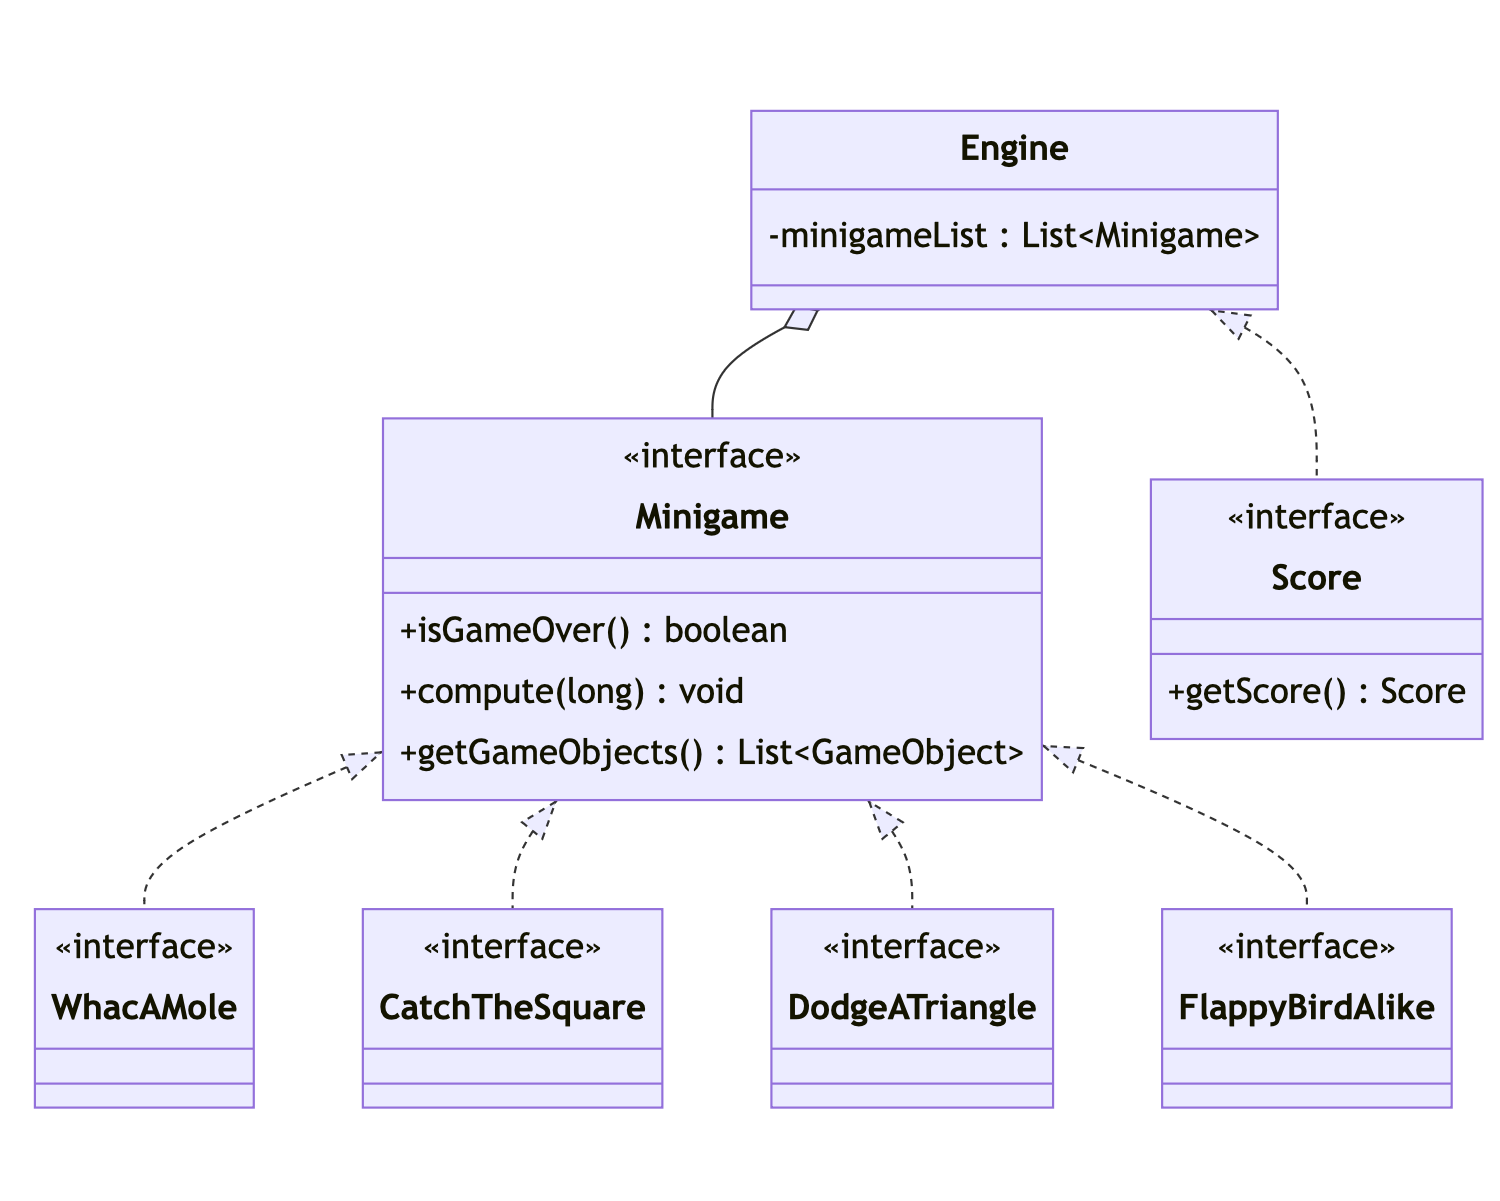
\includegraphics[width=\textwidth]{domain.png}
	\caption{UML diagram of the domain analysis}
\end{figure}

\chapter{Design}

\section{Architecture}
The project is built on the "model-view-controller" architecture: the \textbf{View} will be the entry point of the program.
At its creation it will instantiate the game window and the \textbf{Controller} class.
When the user decides to start the run it will be asked to the controller to create an \textbf{Engine}, this class will manage each \textbf{Minigame}.\\
The Model part is represented by the implementation of \textbf{Minigame}s these will contain \textbf{GameObject}s that will evolve over time with a specific logic.
The \textbf{Controller} directs the run with the game loop pattern, updating each frame the view with the \textbf{GameObject}s fetched from the \textbf{Engine}.
The \textbf{Controller} takes also care of intercepting the user's input from the \textbf{View}, then it forwards it to the Engine.
Once the input has been received, the Engine is responsible for communicating it to each minigame: these in turn will update the state of all the GameObjects they contain, i.e. every single entity in the various playing fields.

\section{Detailed design}
\textbf{Problem:} Each GameObject must have a specific aspect and behaviour\\
\textbf{Solution:} Each minigame is composed of \textbf{GameObject}s: those items use a component pattern, thanks to which we get
a full separation of concerns based on domains (allow a single entity to span multiple domains each other\footnote{From GPP, CH 14}).
\pagebreak
\begin{itemize}
	\item \textit{PhysicsModel}: Interface that deals with the physical state of a Game Object,
	      moving it according to its speed, considering the environment in which it is located (edges of the field)
	      and the other objects it interacts with (collision with obstacles).
	\item \textit{AspectModel}: It is the interface that sets the look of the single\\ \textbf{GameObject}, specifying which of the Drawing instructions need to be used.
	\item \textit{InputModel}: Interface related to a single GameObject that reads the input stored in the
	      engine and applies it, if the object recognizes it as its own command, changing its specifications (e.g. coordinates, speed).
	\item \textit{HitBoxModel}: Defines the shape and sizes of the hitbox that the object shall interpret when colliding with other hitboxes.
\end{itemize}

\begin{figure}[ht]
	\centering{}
	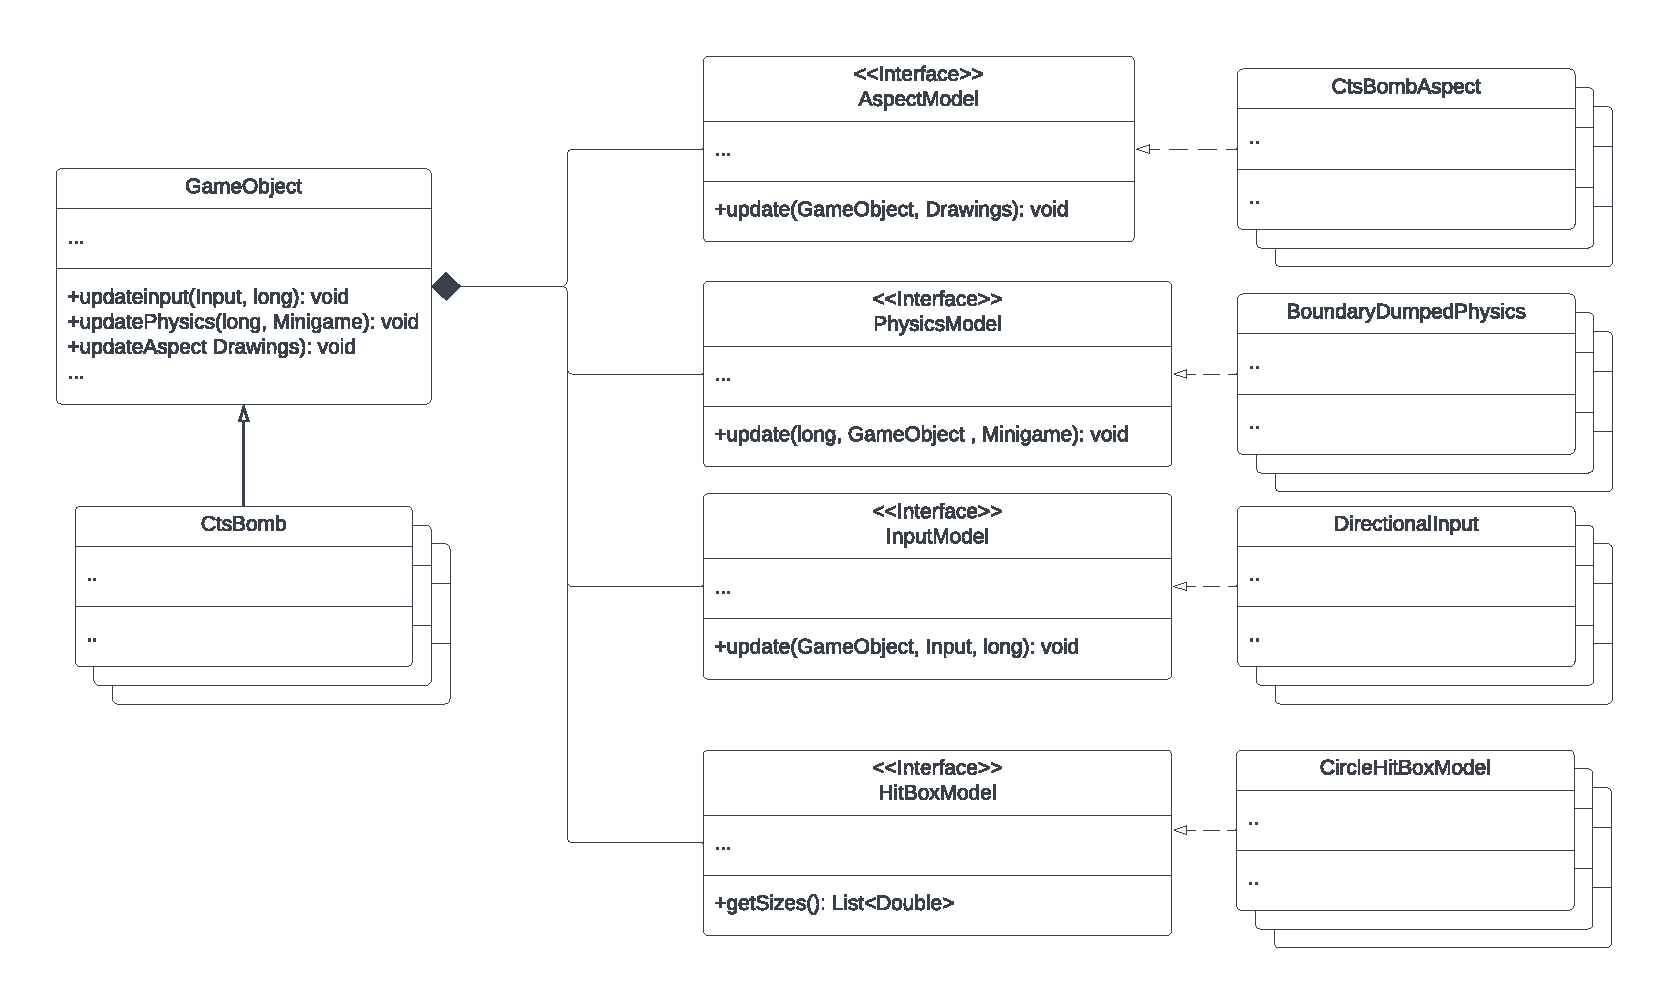
\includegraphics[width=\textwidth]{res/componentPattern.pdf}
	\caption{UML diagram of the component pattern}
\end{figure}
\subsection*{Leonardo Tassinari}
\textbf{Difficulty in CTS}\\
\textbf{Problem:} The spawn rate of the squares shall increase over time.\\
\textbf{Solution:} The CatchTheSquare's constructor adopts the strategy pattern taking a \textit{Function} interface. That function will return to the minigame the number of bombs that are expected to be spawn so far given the total amount of milliseconds elapsed from the beginning of the minigame.
My implementation of the function uses an exponential curve to increment the spawn rate progressively until a certain rate.
The limit rate is represented by the inclination of the line tangent to the exponential curve on the point where the derivate of the exponential reaches that steepness.\\
\begin{figure}[ht]
	\centering
	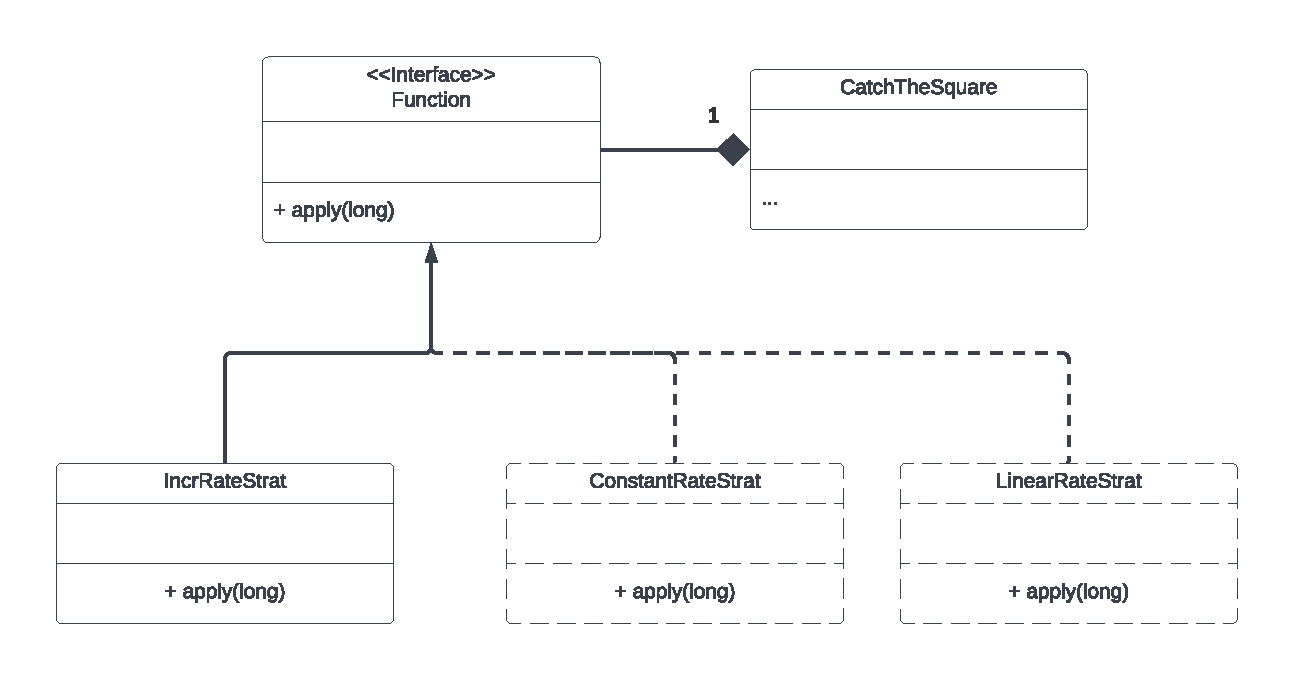
\includegraphics[width=\textwidth]{res/RateStrat.pdf}
	\caption{The corresponding UML diagram}
\end{figure}
\begin{figure}[ht]
	\centering
	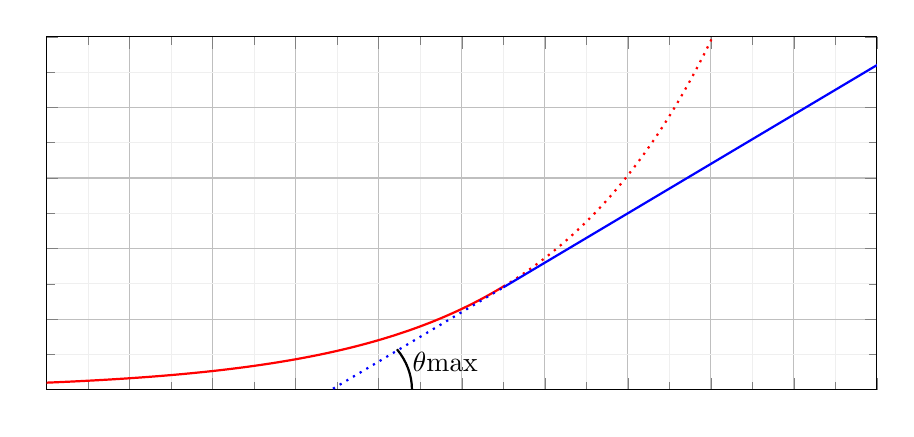
\begin{tikzpicture}
		\begin{axis}[
				xmin = 0, xmax = 100,
				ymin = 0, ymax = 50,
				xtick distance = 10,
				ytick distance = 10,
				xticklabels=\empty,
				yticklabels=\empty,
				grid = both,
				minor tick num = 1,
				major grid style = {lightgray},
				minor grid style = {lightgray!25},
				width = \textwidth,
				height = 0.5\textwidth
			]
			\addplot[
				domain = 0:55,
				samples = 200,
				smooth,
				thick,
				red,
			] {1.05^x};
			\addplot[
				domain = 55:150,
				samples = 200,
				dotted,
				thick,
				red,
			] {1.05^x};
			\addplot[
				domain = 55:150,
				samples = 200,
				smooth,
				thick,
				blue,
			] {x*0.7-24};
			\addplot[
				domain = 0:55,
				samples = 200,
				dotted,
				thick,
				blue,
			] {x*0.7-24};
			\pgfmathsetmacro{\angle}{asin(0.7/sqrt(1+0.7^2))} %asin(rise/hypotenus)
			\draw[black,thick] (axis cs: 44, 0) arc[start angle=0, end angle=\angle, radius=10];
			\node[black] at (axis cs: 48, 4) {\(\theta\)max};
		\end{axis}
	\end{tikzpicture}
	\caption{An example of the trend of the implemented function}
\end{figure}
\pagebreak\\
%\textbf{Collider}\\
%\textbf{Problem:} In more minigames is required to check collisions between two objects.\\
%\textbf{Solution:} A public utility class to check collisions between object's hitboxes.
%\begin{figure}[ht]
%	\centering
%	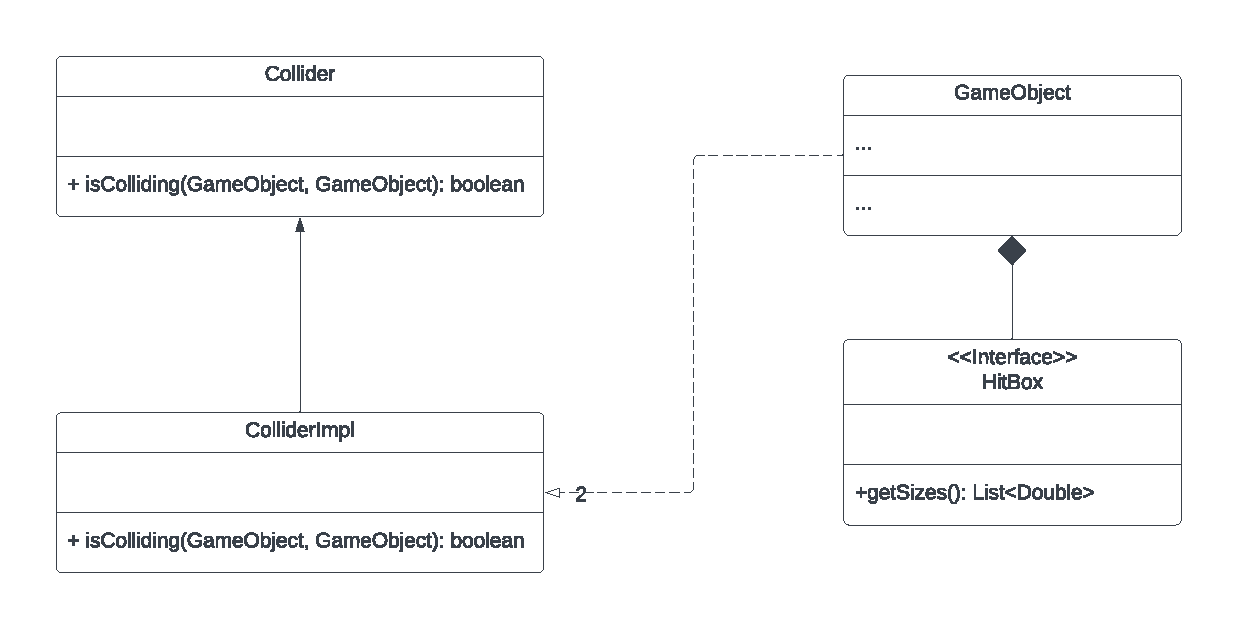
\includegraphics[width=\textwidth]{res/Collider.pdf}
%	\caption{The UML diagram of the Collider}
%\end{figure}\\
\textbf{Button Factory}\\
\textbf{Problem:} In the whole user interface is required a consistent look and feel of the buttons.\\
\textbf{Solution:} By encapsulating the creation of buttons in the \textit{ButtonFactory} class, it is ensured that all buttons created through this class have the same visual style, and can be easily modified in one place if needed while also taking care of some of the underlying complexities of button creation such as sizing and styling.
\begin{figure}[ht]
	\centering
	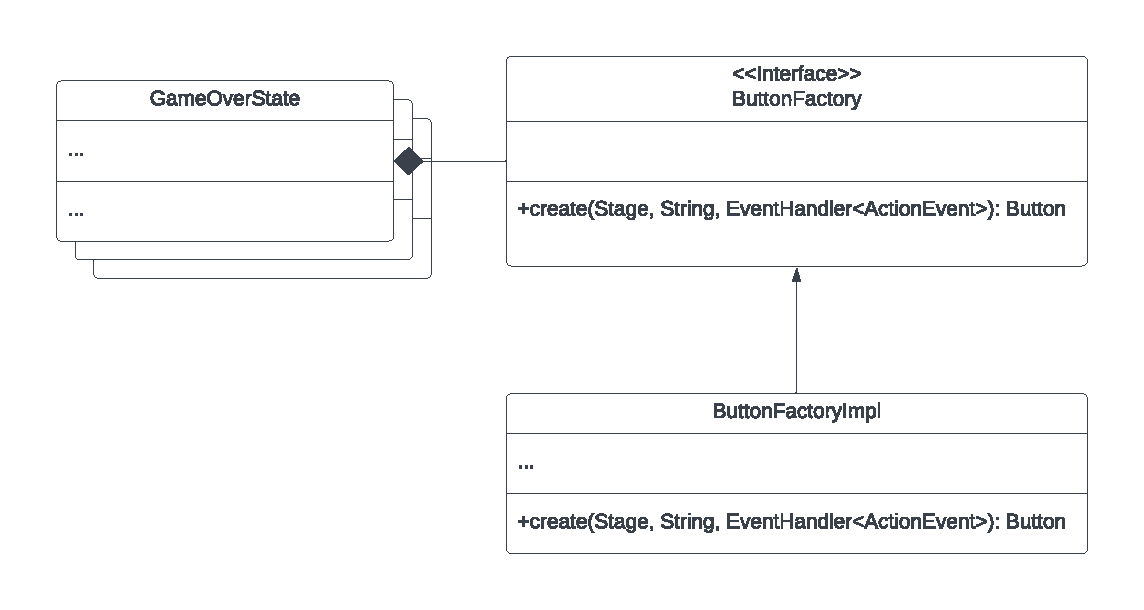
\includegraphics[width=\textwidth]{res/ButtonFactory.pdf}
	\caption{The UML diagram of the ButtonFactory}
\end{figure}\\
\textbf{View States}\\
\textbf{Problem:} The \textit{View} shall display different items over time.\\
\textbf{Solution:} The \textit{JavaFxView} adopts a state pattern, each state has a method to display its item overwriting the ones present at the moment.\\
A special state, the \textit{GameState} is a subclass of state able to show the gameplay.
\begin{figure}[H]
	\centering
	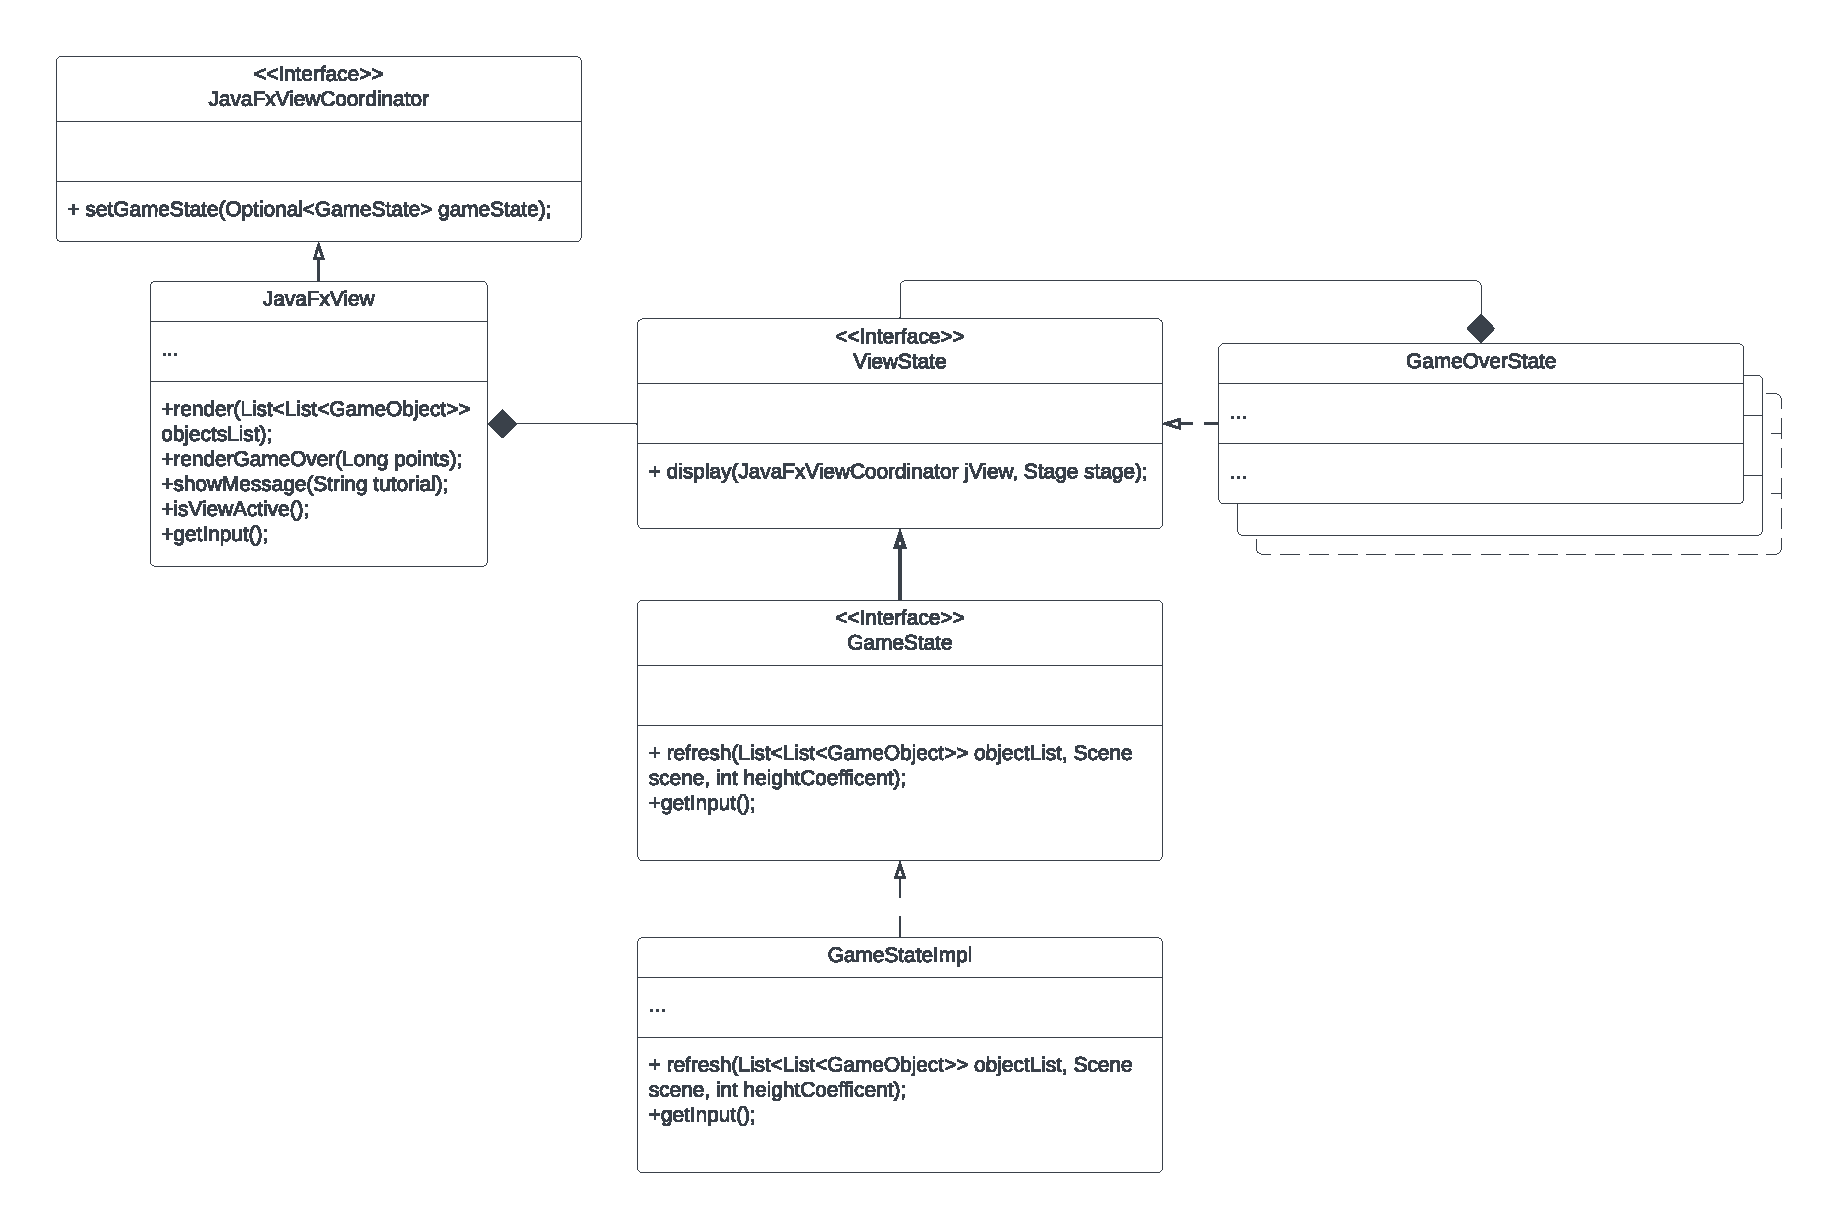
\includegraphics[width=\textwidth]{res/ViewState.pdf}
	\caption{The corresponding UML diagram}
\end{figure}
\pagebreak

\subsection*{Pietro Olivi}
\textbf{Difficulty in WhacAMole}\\
\textbf{Problem:} What is the logic behind the appearance of a Mole or Bomb?\\
\textbf{Solution:} When it came time to deal with the Moles and Bombs spawn problem, as well as providing my own version of the algorithm
I thought it was vital to come up with a solution that would leave room for future changes, i.e. ideas on how to handle the GameObjects’
random extraction. I therefore recognized a natural correspondence with the strategy pattern. Initially I was thinking in terms of time
intervals: At the beginning of each set period I would extract a variable number of objects (also assigning the lair from which to spawn)
so that they would appear by the end of that interval, however so many checks had to be done that the entire lifecycle of Moles and Bombs
did not exceed the right limit of the current interval that the code became unclear. I therefore decided to extract a variable number of
objects, at most equal to the maximum number of GameObjects simultaneously in action, and do it again when all of them had finished their
work (each entity will also have a waiting time before appearing, otherwise it would become impossible).
\begin{figure}[ht]
	\centering
	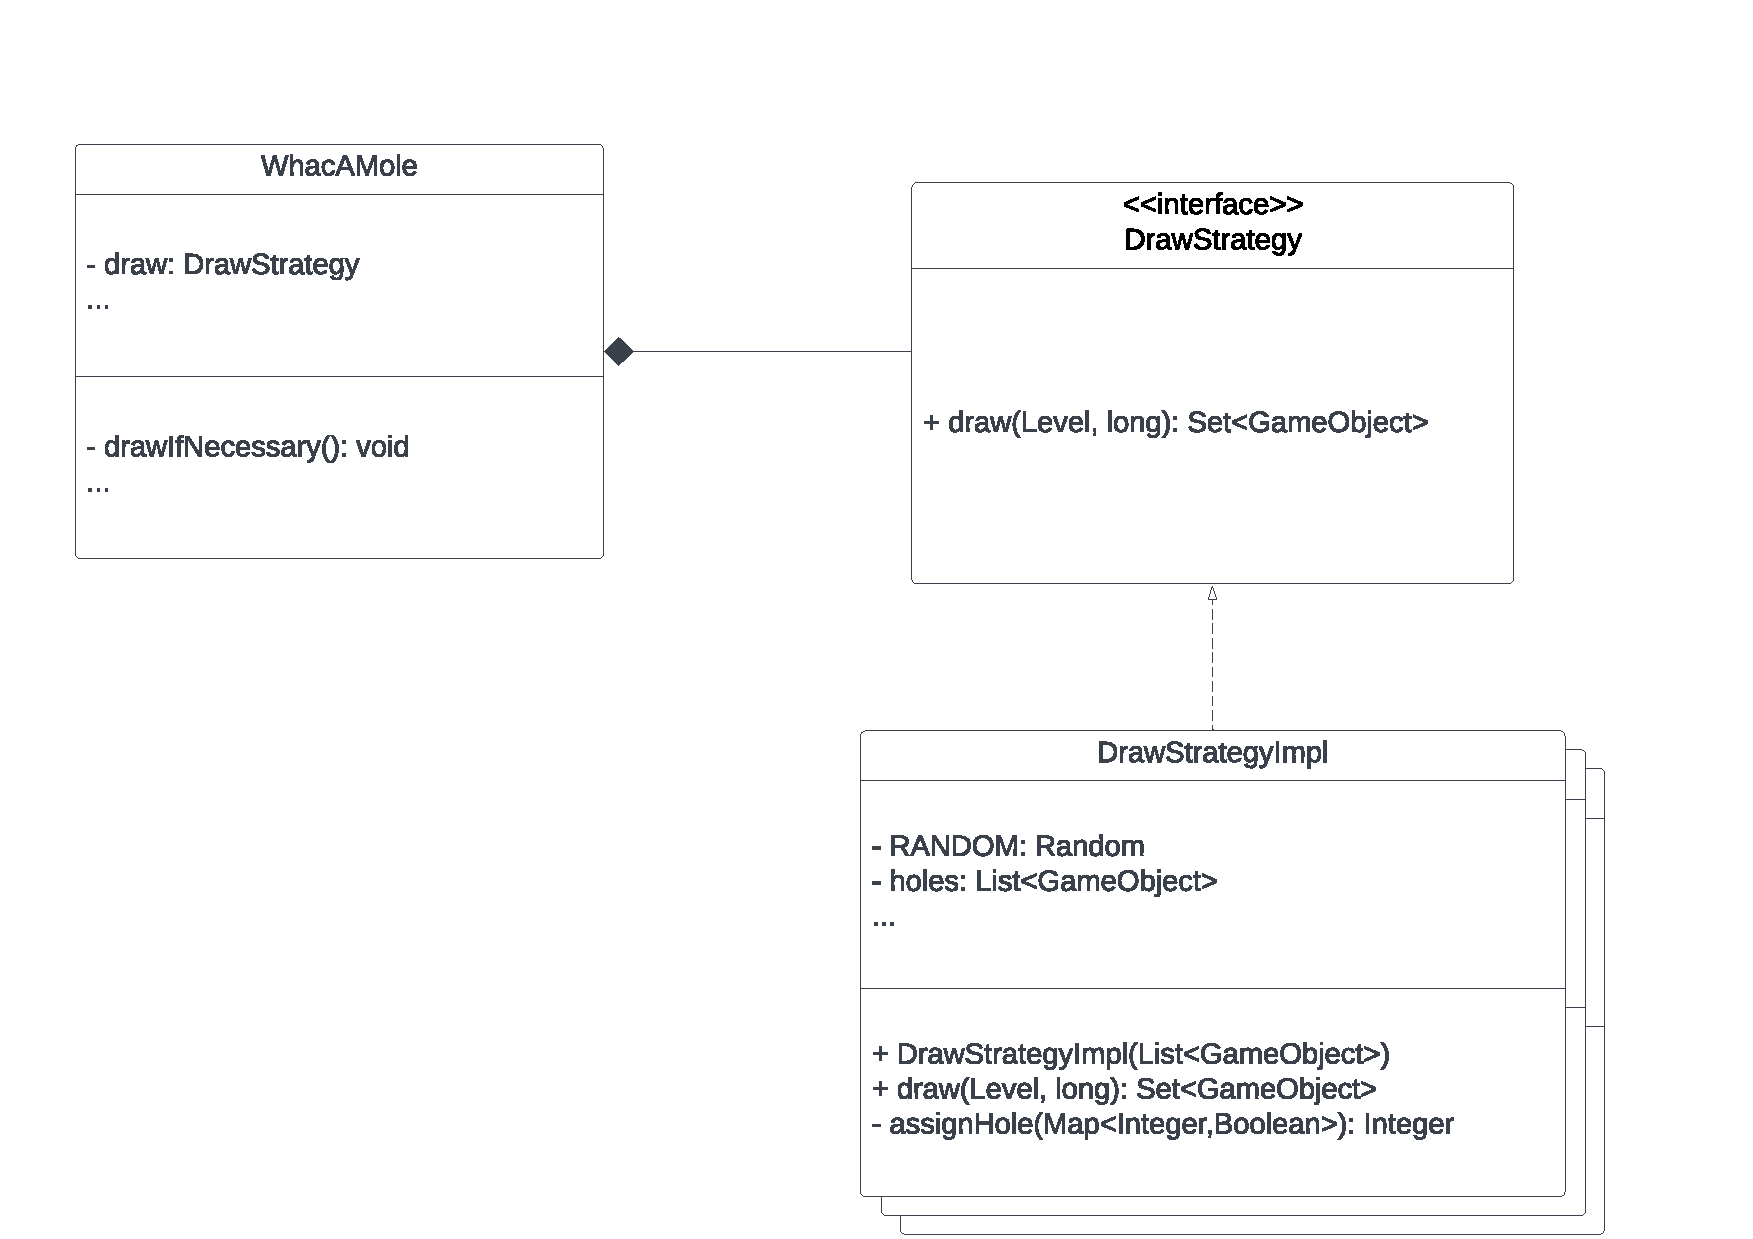
\includegraphics[width=\textwidth]{res/DrawStrategy.pdf}
	\caption{The corresponding UML diagram}
\end{figure}
\pagebreak\\
\textbf{Problem:} Each Mole and Bomb will have to appear in a specific spot on the
pitch, but where?  \\
\textbf{Solution:} The problem of the positioning of the dens is certainly not going to have a single solution, since this strongly depends
on the number of dens with which you intend to play. Taking the classic arcade version of Whac-a-Mole as a reference, I provided an
implementation that distributes the holes equidistantly (into a table), suitable for numbers whose root is an integer. However, wanting to
allow the insertion of other possible positioning strategies, I again leaned on the strategy pattern (although the interface does not appear
as a Whac-a-Mole field but as a variable inside the constructor, being used only there).
\begin{figure}[ht]
	\centering
	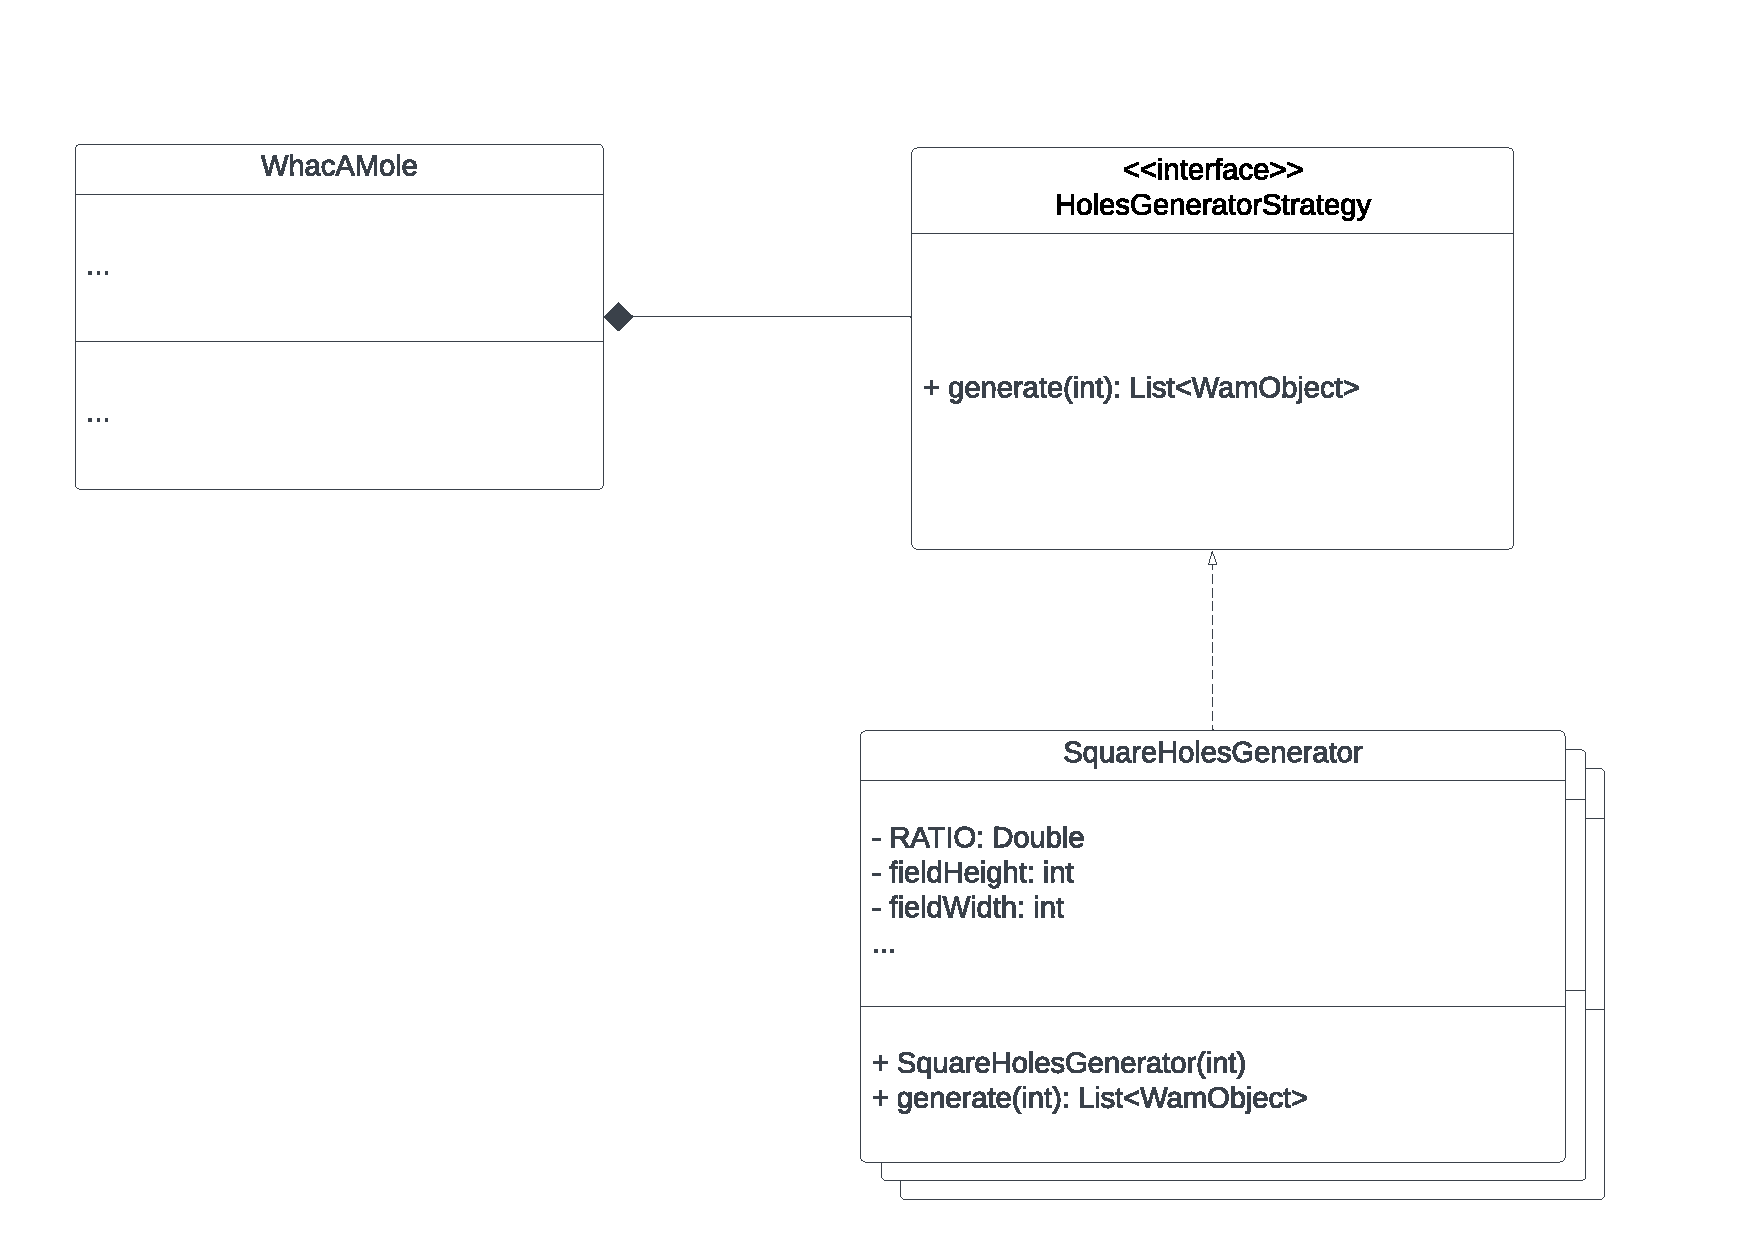
\includegraphics[width=\textwidth]{res/HolesGenerator.pdf}
	\caption{The corresponding UML diagram}
\end{figure}
\pagebreak

\subsection*{Lorenzo Dalmonte}
\textbf{Input in FlappyBirdAlike}\\
\textbf{Problem:} The player action must be performed only when the button is pressed.\\
\textbf{Solution:} The solution I came up with initially was to turn off the specific input if it was on in order to get a result only on the first cycle,
however that wouldn't work since on the following cycle the Input would be turned back on if the player was still holding the key down.
Therefore the InputModel itself had to recognize whether the player is holding down the key. I achieved that by adding a boolean field that's set to true
if the player pressed the key and set to false once the player stopped holding it down.

\pagebreak\\
\textbf{Difficulty in FlappyBirdAlike}\\
\textbf{Problem:} The obstable spawn rate must increase over time.\\
\textbf{Solution:} I wanted to make a steady difficulty increase while making sure the player recognizes the moment the minigame gets tougher.
I needed to simulate a non-continous function that increased linearly, therefore I implemented a step-like function similar to a floor function.
It recieves the total number of elapsed frames since the minigame began and returns an integer, in this case the coordinate the closest obstacle
has to reach before the next one spawns. This increases the spawn frequency of the obstacles until the function returns a max value.

\chapter{Development}
\section{Automated Tests}
We created with Junit 5 the following automated tests:
\begin{itemize}
	\item AesEncryptionImplTest:\\
	      Checks if a test string is correctly encrypted and if it's correctly decrypted.
	\item AesEncryptionImplTestSerializable:\\
	      Checks if a test object serialization is correctly encrypted and if it's correctly decrypted.
	\item BombTest:\\
	      Checks if the bomb's timer decreases.
	\item CatchTheSquareTest:\\
	      Checks if the bomb actually runs out of time.\\If, when run over by the circle, it disappears.\\ If the Input class moves the circle. \\ If the Circle stays inside the boudaries.
	\item IncrRateStratTest:\\
	      Checks if the function steepness is increasing in the first part.\\ If the function is flattenting on the second part.
	\item StepRateStratTest:\\
	      Checks if the output gap between two values is a multiple of the step height.\\ Makes sure the function doesn't go over the maximum value.
	\item FlappyBirdAlikeTest:\\
	      Makes sure the cursor never goes out of bounds.\\ Checks whether the first obstacle in the list is also the closest to the player.\\ Makes sure hitboxes work properly.\\ Makes sure the cursor doesn't move on its own.
	\item DodgeATriangleTest:\\
	      Makes sure hitboxes work properly.\\ Makes sure the player never goes out of bounds.
	\item WhacAMoleTest: \\
	      Checks that a mole, if not hit, causes Game Over. Controls whether hitting it instead will cause the game to continue. The same is done for the bomb, however, checking that if it is hit the game ends and that nothing happens if ignored

\end{itemize}
 \section{WorkFlow}
 We began discussing the needs of the application and planning the architecture, after that we created the backbone of the program making the main interfaces.
 During the Development the adopted strategy for the DVCS was to create a branch for each feature on Development, doing so we limited the merging conflict.
 In that phase the roles were:
\subsection*{Leonardo Tassinari}
\begin{itemize}
	\item Creation of the Catch-The-Square minigame
	\item Creation of the Encrypter tool
	\item Creation of the Collider checker
	\item Implementation of the JavaFxView
\end{itemize}

\subsection*{Pietro Olivi}
\begin{itemize}
	\item Creation of the Whac-A-Mole minigame
	\item Co-Creation of the Dodge-A-Triangle minigame
\end{itemize}

\subsection*{Lorenzo Dalmonte}
\begin{itemize}
	\item Creation of the Flappy-Bird-Alike minigame
	\item Co-creation of the Dodge-A-Triangle minigame
	\item Creation of Record-Loader and stats display
\end{itemize}

\section{Development Notes}
Following, for each member, are listed the advanced aspects of the language that had been used.
\subsection*{Leonardo Tassinari}
\begin{itemize}
	\item Widely used lambda expressions
	\item Reflection
	\item Optional
	\item Stream
	\item JavaFx
	\item javax.crypto.Cipher
	\item Thread
\end{itemize}

\subsection*{Pietro Olivi}
\begin{itemize}
	\item Lambda expressions used extensively (also method references)
	\item Stream (21 in WhacAMole.java and WhacAMoleTest.java combined)
	\item Optional
\end{itemize}

\subsection*{Lorenzo Dalmonte}
\begin{itemize}
	\item Widely used lambda expressions
	\item Stream
	\item JavaFx
\end{itemize}
\chapter{Final Considerations}
\section{Self-Evaluation and future projects}
\subsection*{Leonardo Tassinari}
Even thought it was our first time coping with such a big project,
I have to say that overall we managed to collaborate in a satisfactory way, we were able to share tasks wisely, spread ideas and help each other when needed.
Personally I've enjoyed the most working on the implementation of the model, while on the other hand the most frustrating part has been the planning of the architecture since it led me to some overthinking.
I don't think that the project will receive further support in the future, nevertheless it passed on us very valuable experiences and knowledge.
\subsection*{Pietro Olivi}
As this was my first medium(-large) sized project, it didn't always go very smoothly. As an auticritic I would blame myself for taking a bottom-up approach to my minigame 
feature design. In particular, I found myself "adding pieces" to the core part of the minigame without much forethought, which resulted in me changing the same part 
of code several times, and thus stressing as well as wasting a great deal of time. On the other hand, I think (/hope) I was a clean and careful programmer, always 
straight to the point, able to work in a group effectively. All in all, I am very proud of the final product.
\subsection*{Lorenzo Dalmonte}
This was the first time I've worked on a big project, and it shows a little bit. I didn't always face this project as I should have. Instead of following a smooth schedule
until the final deadline, I mostly worked a lot in short amounts of time leaving big gaps in between. Even though I didn't approach the project in the best way, I still think
it turned out great and I've enjoyed working on it together with the team. This definitely helped me understand how to work efficiently in groups.

\section{Difficulties faced and comments for the teachers}
\subsection*{Leonardo Tassinari}
The only point I'd like to raise here is regarding how the correction of the lab practices is managed in class: each time you complete an exercise you have to raise your hand and wait for an undefined amount of time.
So my suggestion is to have more tutors and implement a structured queue (with an app maybe) in order to avoid people skipping the line.
\subsection*{Pietro Olivi}
Nothing to say about teaching, but I would have some doubts about the amount of work that this course requires to be "only" 12 credits. The project turned out to be fundamental for learning the subject and a first 
contact with the world of software engineering, but I don't find it fair that this happens to the detriment of other equally important subjects in the semester following that of the lessons (on which the project falls), 
from which a lot of time is taken away, finding us having to follow 4 subjects, with their respective possible projects, plus OOP. As a consequence, during the lessons of the second semester of the second year you can 
see the vast majority of the class writing code in java rather than listening. For comparison, at the end of the lessons, the amount of material and the hours of lessons were more or less the same as for Operating Systems 
(12 credits), but for OOP there were 80 hours of actual individual work left to do.
\subsection*{Lorenzo Dalmonte}
I don't have any complains regarding the lessons however, as my teammates already discussed, this course requires a substantial amount of work that, for many students,
hinders the learning of other subjects which are just as important. Even though this may sound like a problem due to poor time management on our end (which might be the case for a few students),
I personally think that even with close to perfect planning the OOP project will still take away some time from other subjects.


\appendix
\chapter{User Guide}
At the start of the program a window will appear, you can move and resize it to fit best your situation, you can also {\color{red}switch to full screen mode by pressing the "F" key}.
\section*{Whac-A-Mole}
Moles and Bombs will randomly appear on the playing field: sufficient conditions for losing the game are to let a mole return to its
burrow without being crushed, or to hit a bomb. If you are using a keyboard with horizontal arrangement of numbers, to hit an object that
is outside the hole, just press the number corresponding to the latter. In particular, the dens will be numbered in ascending order starting
from the first in the upper left, continuing towards the right, and then moving on to the first in the next row (once the previous one is
finished). If you have a numpad available then, in the case of the standard 9-hole version of the game, you will have to press, more intuitively,
the key in the position corresponding to that of the lair.
\begin{figure}[!htbp]
	\centering{}
	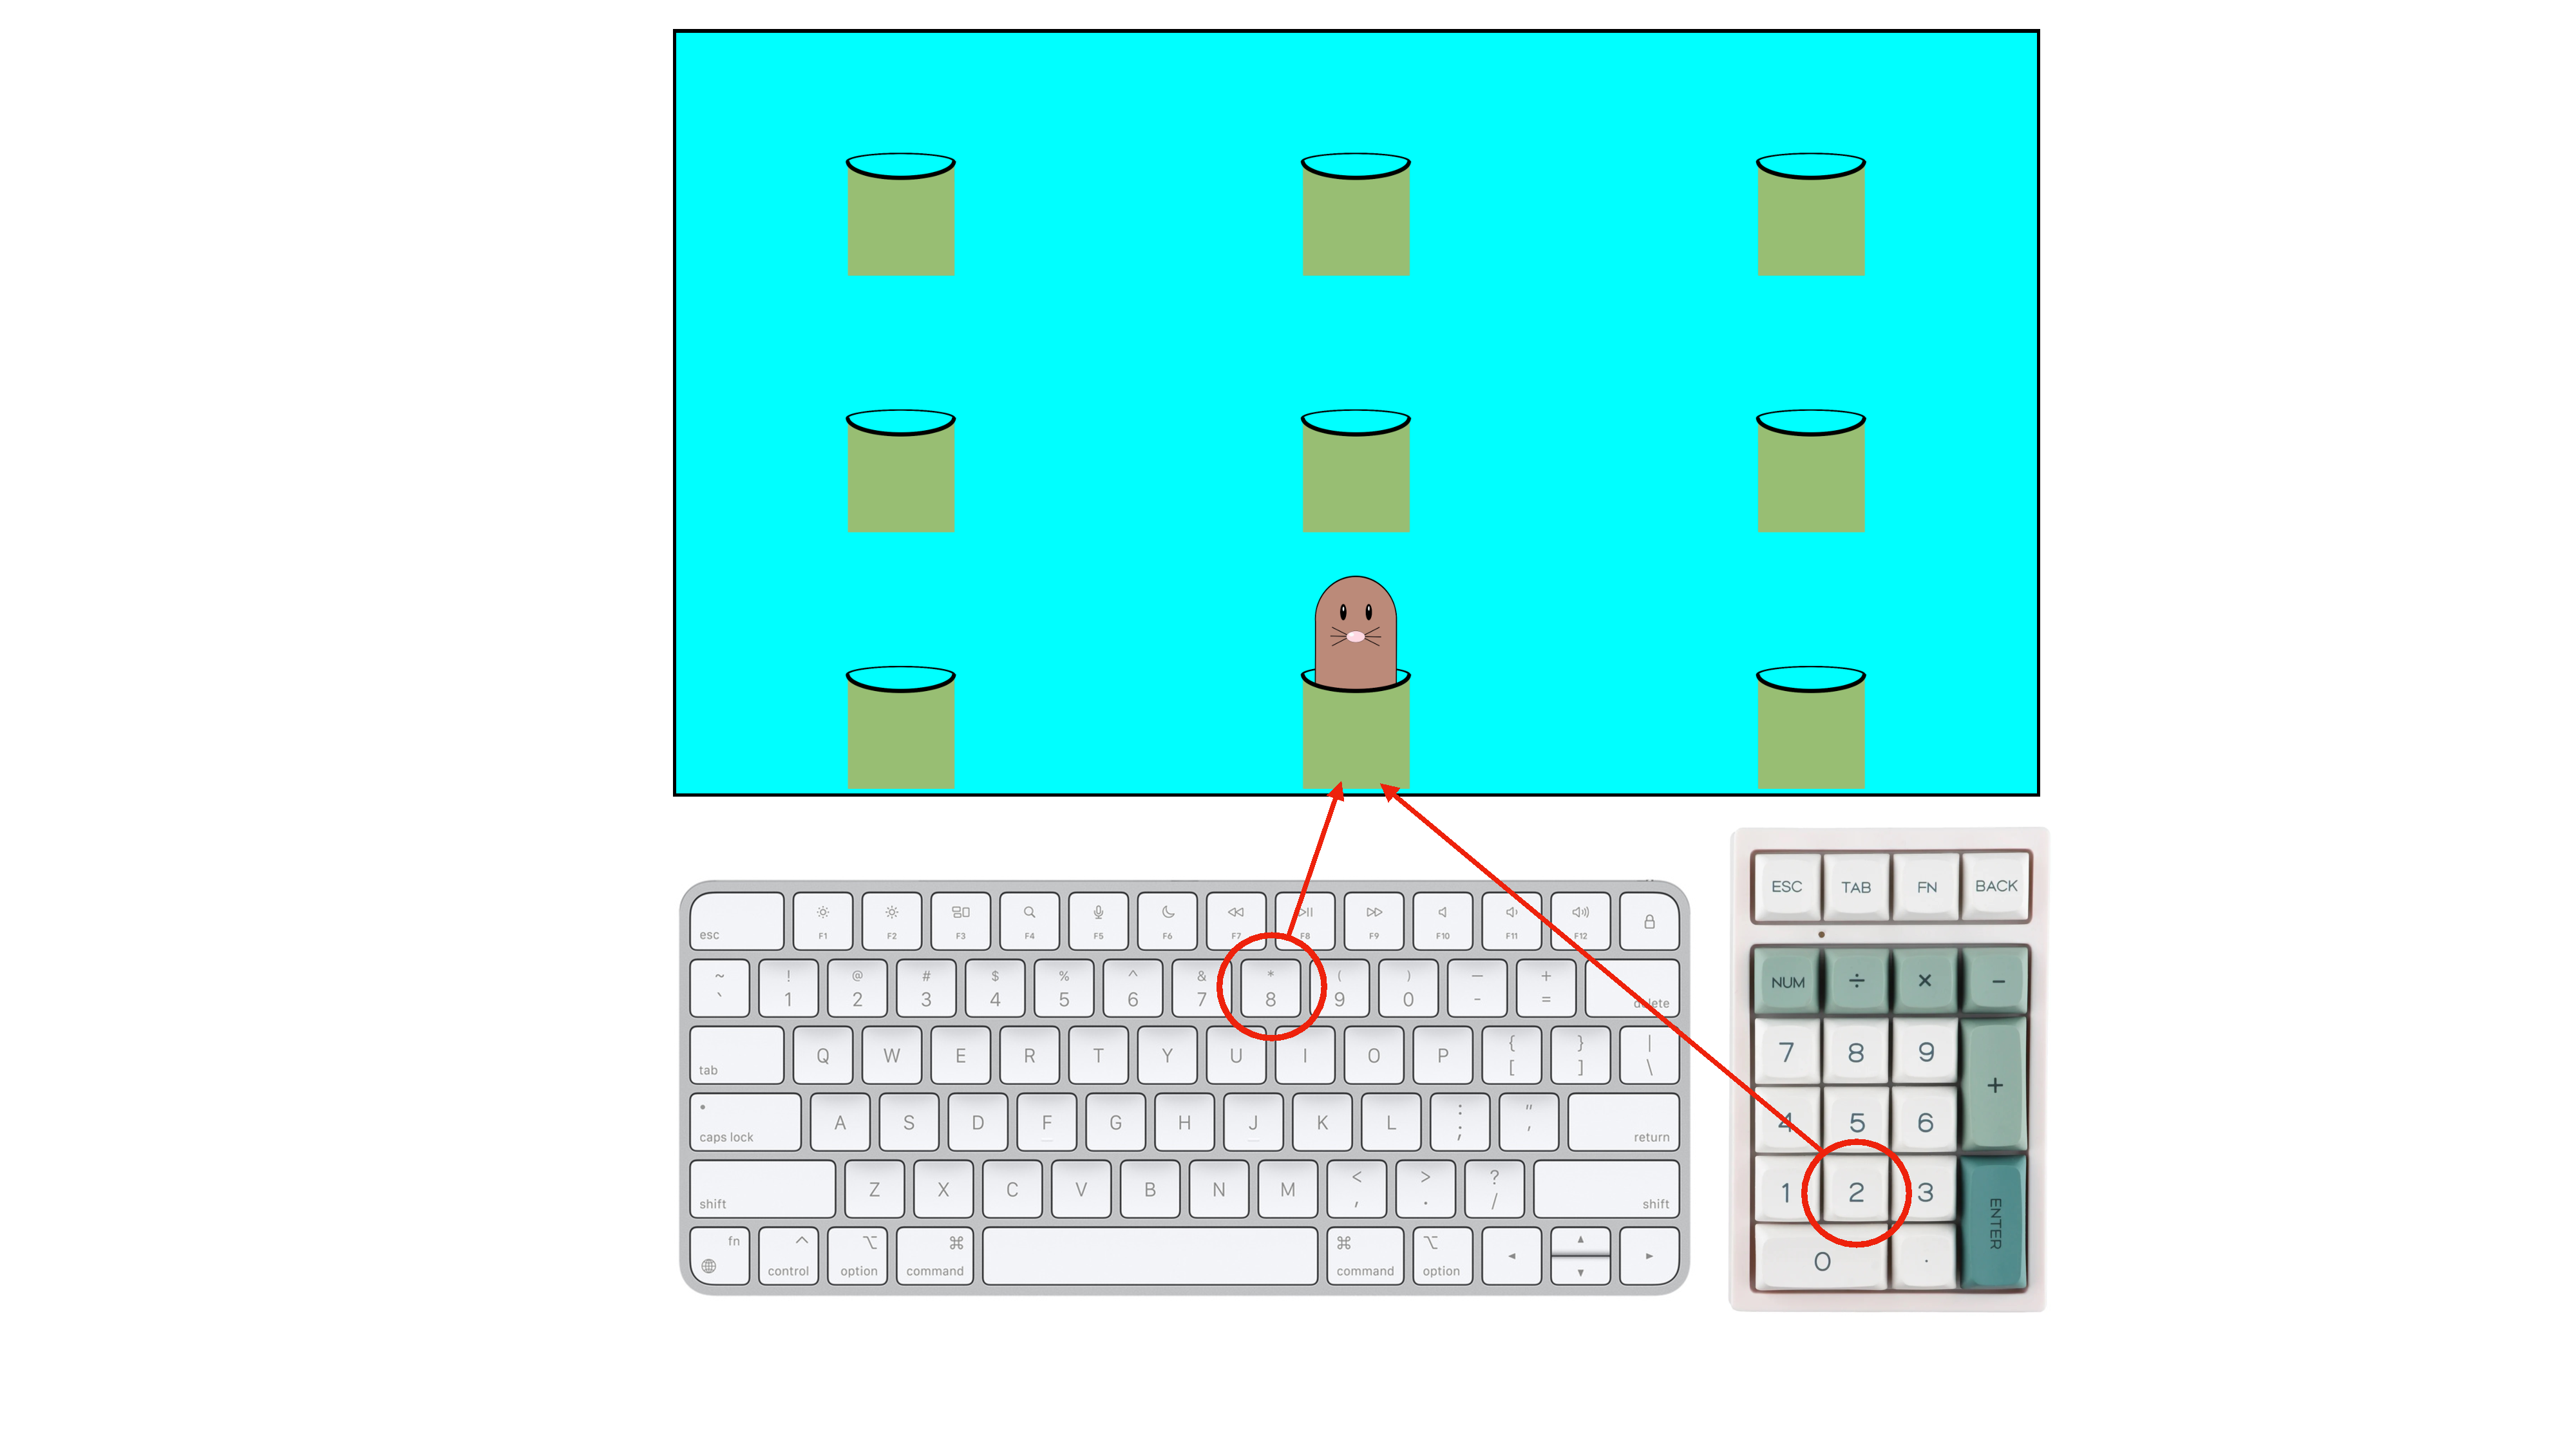
\includegraphics[width=\textwidth]{res/InstructionsWam.pdf}
	\caption{Keys to use to play Whac-a-mole}
\end{figure}
\section*{Catch-The-Square}
You will control a circle with the "WASD" keys, moving it on the pane, your objective is to hit the spawing squares to remove them, each square has a timer, don't let it run out!\\
When you bounce on the walls yours speed will be dumped, therefore you cannot gain high speed and forget this minigame.
With time the spawn rate of the squares will increase, good luck!
\begin{figure}[H]
	\centering{}
	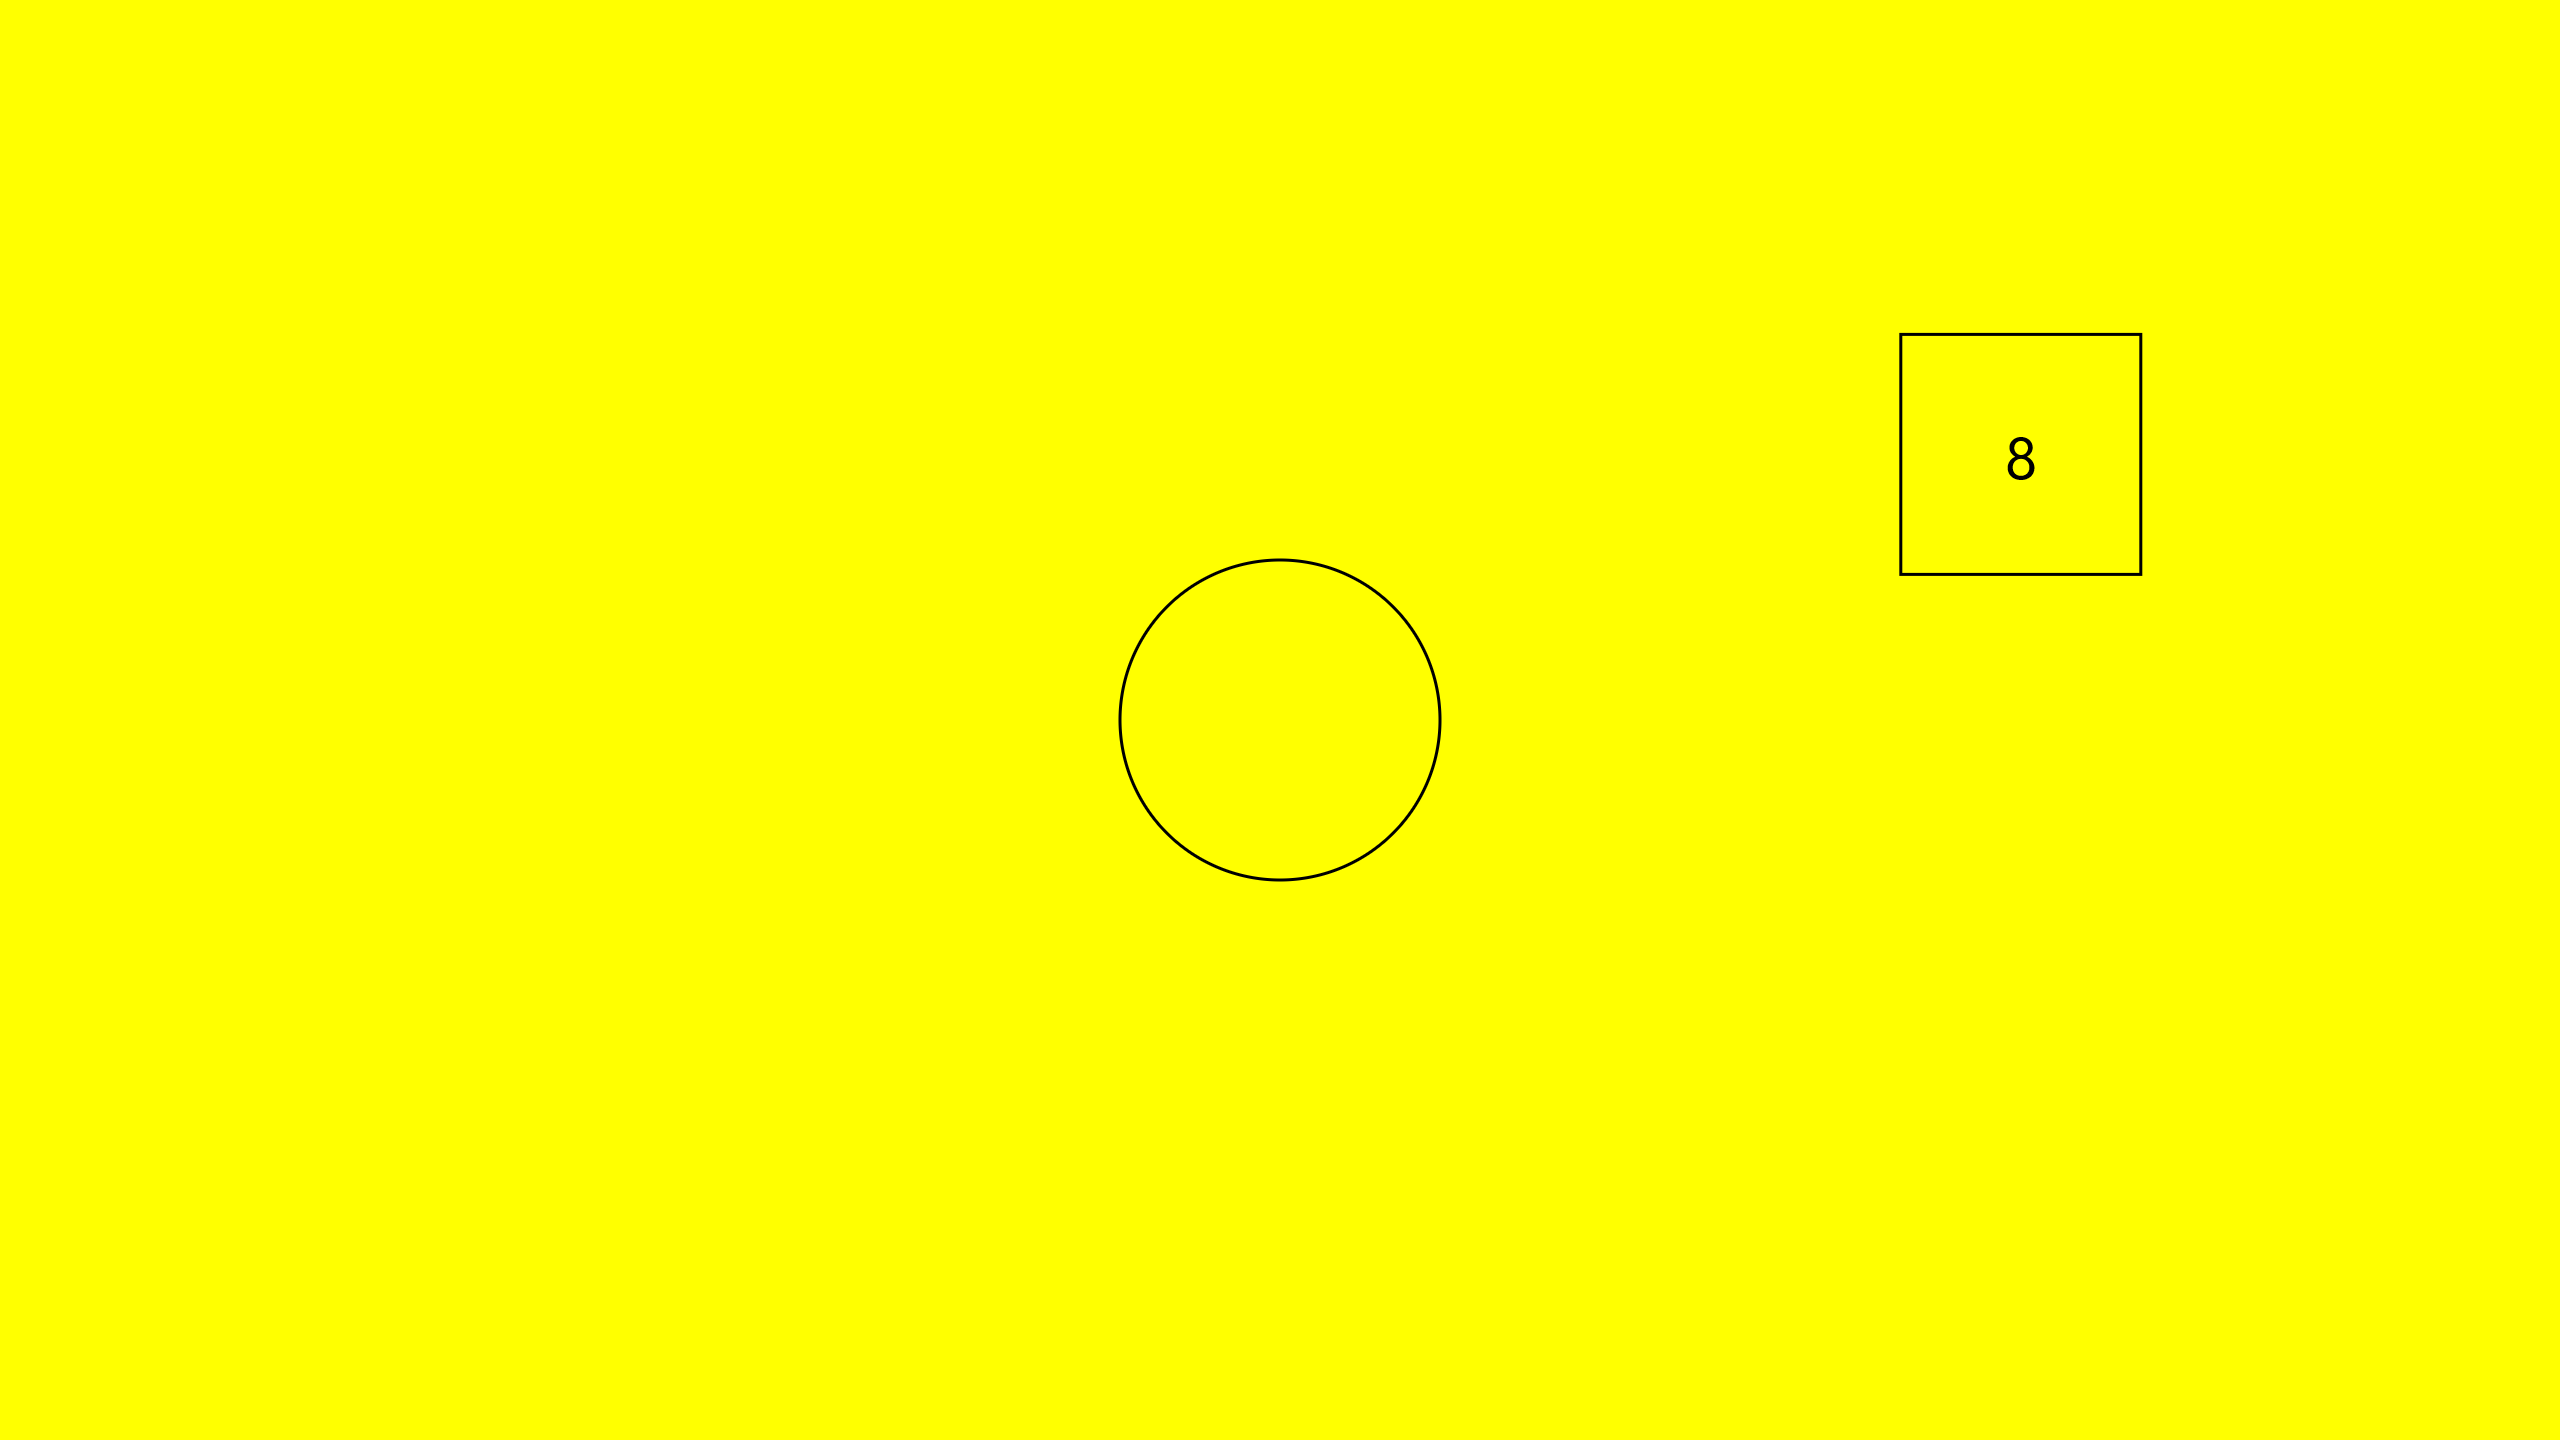
\includegraphics[width=330pt]{res/Cts.png}
	\caption{Representation of Catch-The-Square}
\end{figure}
\section*{Flappy-Bird-Alike}
The player controls a triangle shaped cursor on the left side of the screen.\\
Press the SPACEBAR to jump and evade obstacles incoming from the other side. You can jump in midair too!
\begin{figure}[H]
	\centering{}
	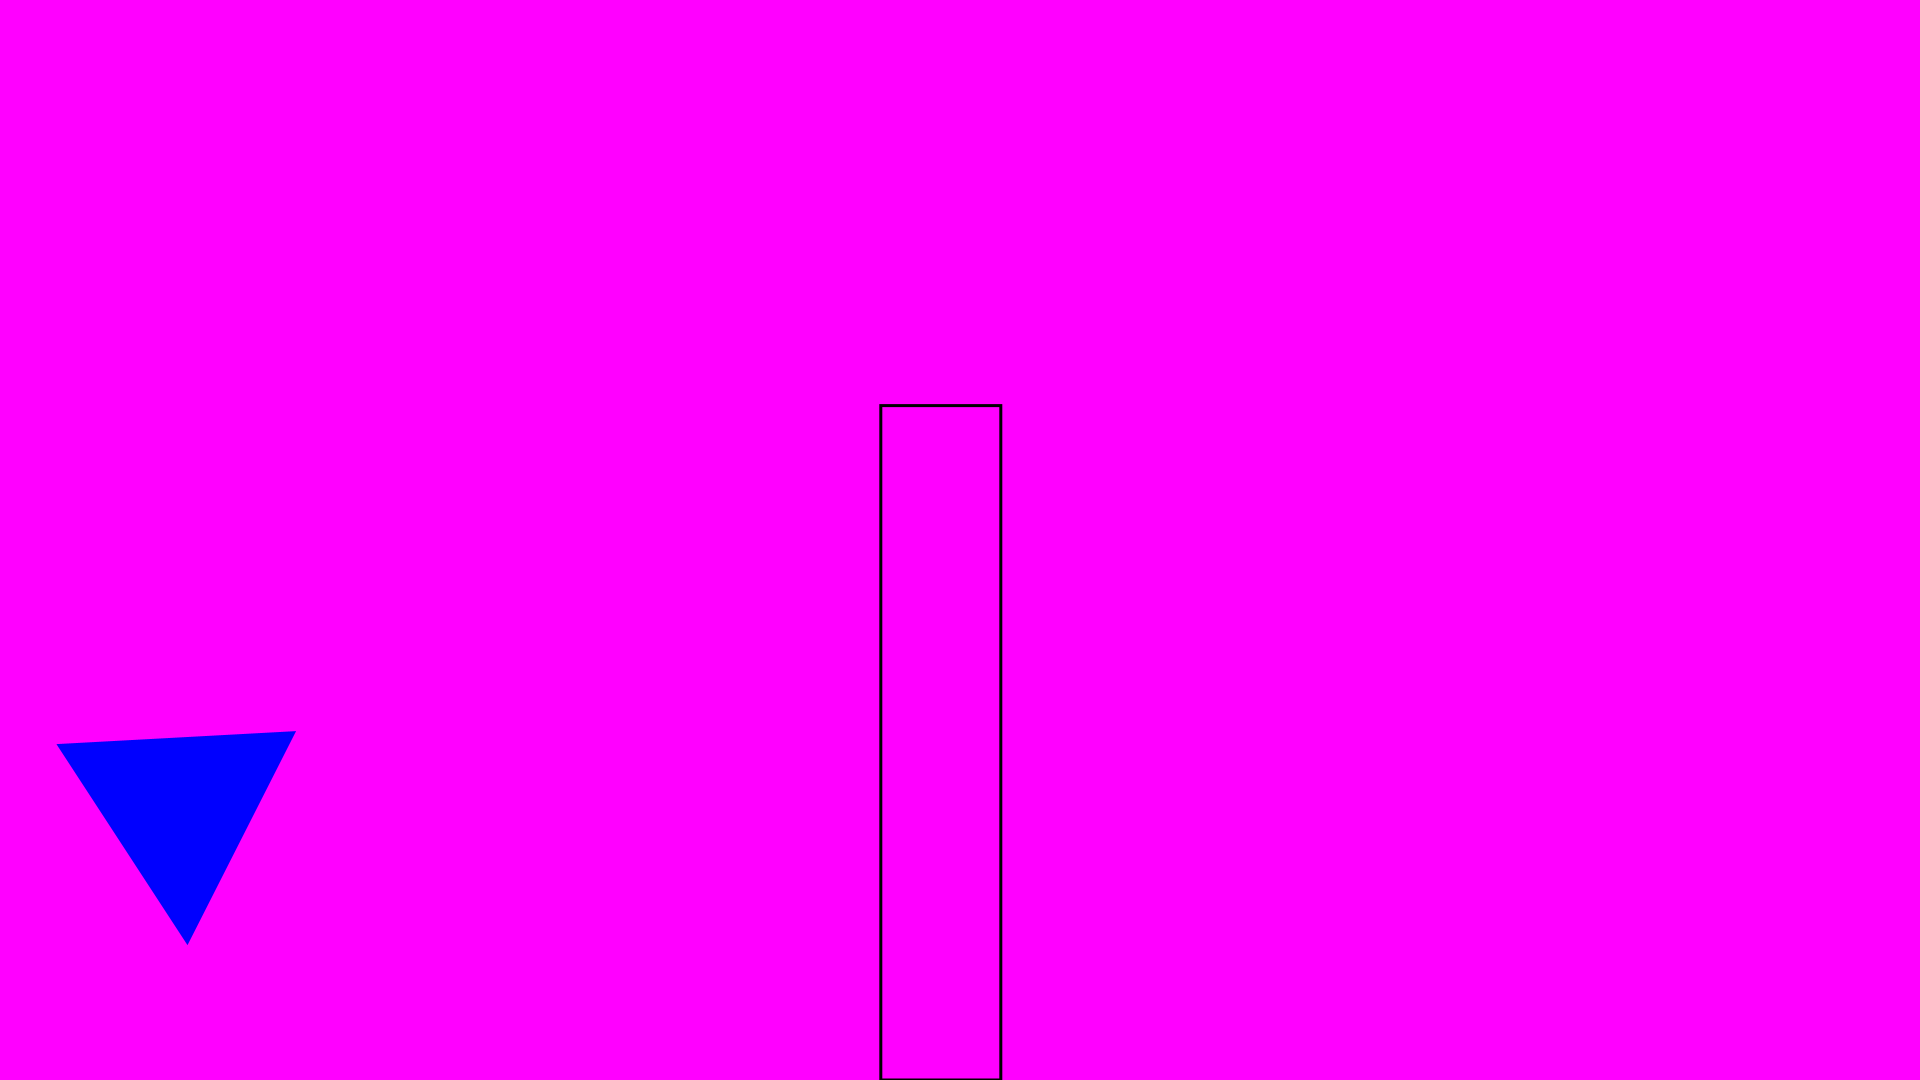
\includegraphics[width=330pt]{res/Fba.png}
	\caption{Representation of Flappy-Bird-Alike}
\end{figure}

\section*{Dodge-A-Triangle}
The player controls a square that moves up and down lanes by pressing the UP and DOWN arrows respectively on the keyboard.\\
Avoid triangle enemies coming from the sides of the screen.

\chapter{Developer Guide}
\section*{Creation of a new minigame}
To create a new \textit{Minigame} you can implement its interface.
Each minigame will keep an internal list of \textit{GameObjects}, that will be updated each frame in 3 main phases:
\begin{itemize}
	\item input process
	\item update
	\item render
\end{itemize}
Each GameObject is composed of Modules regarding different aspects of the object.
You can create your own modules or use the ones already present, take a look at the javaDoc for a more comprehensive list.
\section*{Input Process}
At each frame An Input class is given to each GameObject, it can fetch from it with the getters all the relevant inputs.
You can edit the \textit{Input} Interface and the corresponding implementation to add your specific needs.\\
To implement a key pressing if you are using the JavaFxView implementation you have to add instructions to \textit{InputButtonsImpl} in order to edit the Input class that will be forwarded to each GameObject.

\section*{Update}
At every frame this instruction tells the minigame to "move forward in time" the model of the time elapsed from the last frame. It is also supposed \footnote{depending on the implementation} to activate the PhysicsModel of every GameObject in the minigame.
This phase will make the minigame evolve.
\section*{Render}
To allow the rendering you'll be required to implement the "getObjects" method in this way you'll send the list of GameObjects you want to render, in a specific 
composition order. The View will call the \textit{AspectModel} of each GameObject in order to display them. So you can apply a specific look to an object by calling 
the relative instructions of the \textit{Drawings} interface from the AspectModel. The \textit{Drawings} interface contains all the possible aspects types that you 
can display, so after adding a new method you'll have to create the relative implementation. An \textit{AspectModel} can call multiple methods of the \textit{Drawings} 
to create a specific appearance.
\\\\
\textbf{You can find further information and details on the auto generated JavaDoc.}
\chapter{Lab Practices}
\section*{pietro.olivi2@studio.unibo.it}
\begin{itemize}
	\item Lab 05: \url{https://virtuale.unibo.it/mod/forum/discuss.php?d=114647#p169720}
	\item Lab 06: \url{https://virtuale.unibo.it/mod/forum/discuss.php?d=115548#p171327}
	\item Lab 07: \url{https://virtuale.unibo.it/mod/forum/discuss.php?d=117044#p173090}
	\item Lab 09: \url{https://virtuale.unibo.it/mod/forum/discuss.php?d=118995#p175807}
\end{itemize}

\section*{lorenzo.dalmonte4@studio.unibo.it}

\begin{itemize}
	\item Lab 06: \url{https://virtuale.unibo.it/mod/forum/discuss.php?d=115548#p170779}
	\item Lab 07: \url{https://virtuale.unibo.it/mod/forum/discuss.php?d=117044#p172448}
	\item Lab 08: \url{https://virtuale.unibo.it/mod/forum/discuss.php?d=117852#p173898}
	\item Lab 09: \url{https://virtuale.unibo.it/mod/forum/discuss.php?d=118995#p175820}
	\item Lab 10: \url{https://virtuale.unibo.it/mod/forum/discuss.php?d=119938#p176290}
\end{itemize}
\section*{leonardo.tassinari6@studio.unibo.it}

\begin{itemize}
	\item Lab 04: \url{https://virtuale.unibo.it/mod/forum/discuss.php?d=113869#p169260}
	\item Lab 05: \url{https://virtuale.unibo.it/mod/forum/discuss.php?d=114647#p169543}
	\item Lab 06: \url{https://virtuale.unibo.it/mod/forum/discuss.php?d=115548#p171093}
	\item Lab 07: \url{https://virtuale.unibo.it/mod/forum/discuss.php?d=117044#p172618}
	\item Lab 08: \url{https://virtuale.unibo.it/mod/forum/discuss.php?d=117852#p173682}
	\item Lab 09: \url{https://virtuale.unibo.it/mod/forum/discuss.php?d=118995#p174740}
	\item Lab 10: \url{https://virtuale.unibo.it/mod/forum/discuss.php?d=119938#p176083}
	\item Lab 11: \url{https://virtuale.unibo.it/mod/forum/discuss.php?d=121130#p177362}
	\item Lab 12: \url{https://virtuale.unibo.it/mod/forum/discuss.php?d=121885#p178213}


\end{itemize}


\end{document}
